
\section{Definition}

A second problem is the following,

Let $V = \left\{{v_1 , \cdots , v_n }\right\}$ be a set equipped with an unknown linear order. Given a subset of the relations $v_i \leq v_j$, determine the complete linear order by queries of the form: ``is $v_i \leq v_j$ ?''. (\cite{cardinal2013sorting})


\begin{figure}
	\centering
	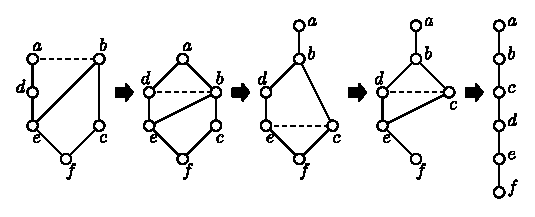
\includegraphics[width=0.7\textwidth]{fig/supi/ex1}
	\caption{\label{fig:supi/ex1} An instance of the problem of sorting under partial information. In this example, we use 4 comparisons (dashed edges). At every step, the Hasse diagram of the currently known partial order is shown. (\cite{cardinal2013sorting})}
\end{figure}
